\documentclass[12pt]{article}
\usepackage[a4paper, portrait, margin=0.5in]{geometry}

\usepackage[T1]{fontenc}
\usepackage[utf8]{inputenc}
\usepackage[english,polish]{babel}
\usepackage{lmodern}
\selectlanguage{polish}

\usepackage{tabularx}
\usepackage{graphicx}
\usepackage{enumitem}

\begin{document}
\newcolumntype{C}[1]{>{\centering\arraybackslash}p{#1}}

\title{Akademia ETI\\\large Instrukcja do laboratorium}
\author{Jan Olencki, Jakub Gierowski,\\Mikołaj Barcikowski, Maciej Brzeski}
\date{27 lutego 2019}
\maketitle
\part{Wprowadzenie}
Tutaj opis logowania
\newpage
\part{Zadania}
\section{Połączenia logiczne}
Zrealizuj funkcję logiczną: \\
\centerline{$f(A,B,C,D)=\overline{A \cdot B + \overline{C+D}}$}
\\
\newpage
\section{Dzielnik częstotliwości}
\subsection{Teoria}
W tym zadaniu poruszony zostanie temat dzielnika częstotliwości. Do obserwacji jego działania zostanie użyta zwykła dioda. Częstotliwość generowana przez urządzenie to 50MHz, co oznacza, że dioda powinna migać co około $2 \cdot 10^{-8}$s, co jest niemożliwe do zauważenia dla człowieka. Jednak poprzez zastosowanie odpowiedniego układu jakim jest dzielnik częstotliwości, można zwiększyć ten czas do np. 1s.
Dzielnik częstotliwości jest układem służącym do zmniejszenia częstotliwości. Układ ten, dzieli częstotliwości zegara wejściowego, czyli częstotliwość generowaną przez urządzeniu i na wyjściu uzyskujemy odpowiednio podzieloną wartość. W układzie przedstawionym na zajęciach oprócz wejścia i wyjścia występuje przycisk reset. Działa on asynchronicznie, czyli wartość na wyjściu ukłądu zostanie wyzerowana w momencie naciśnięcia przycisku, niezależnie od zegara.
\subsection{Krok po kroku}
Lorem ipsum sit dolor amet.
\newpage
\section{Przerzutnik typu JK}
\subsection{Teoria}
\begin{table}[h!]
\renewcommand{\arraystretch}{1.5}
\begin{center}
\begin{tabular}{C{0.6in}|C{0.3in}|C{0.3in}|C{0.3in}|C{0.3in}}
\hline
\hline
$CLK$ & $J$ & $K$ & $Q$ & $\overline{Q}$	\\
\hline
$0 \rightarrow 1$ & 0 & 0 & $Q$ & $\overline{Q}$ \\
$0 \rightarrow 1$ & 0 & 1 & 0 & 1 \\
$0 \rightarrow 1$ & 1 & 0 & 1 & 0 \\
$0 \rightarrow 1$ & 1 & 1 & $Q$ & $\overline{Q}$ \\
\hline
\hline
\end{tabular}
\caption{Tabela wzbudzeń przerzutnika typu JK.}
\label{tab:table1}
\end{center}
\renewcommand{\arraystretch}{1}
\end{table}
Tablica prawdy pokazuje, jaka wartość będzie na wyjsciu przerzutnika(Q) w zalezności od jego wejść J i K oraz sygnału zegarowego CLK. Wartość 1 oznacza stan wysoki, a wartość 0 stan niski. Przerzutnik pracuje w takt zegara, kiedy zmienia się zbocze sygnału zegarowego, czyli kiedy wartość zmienia się z 0 na 1.
\subsection{Krok po kroku}
\begin{enumerate}[wide, labelwidth=!, labelindent=0pt]	
\item Ze strony pobrać plik flipflop.
\item Należy uruchomić program Xilinx ISE 10.1
\item Utworzyć nowy projekt poprzez File/New Project. Upewnić się, że został wybrany folder taki jak na rysunku. Podać nazwę projektu i wybrać z rozwijanego menu Schematic, nacisnąć przycisk Next, a następnie ustawić parametry tak jak na rysunku.\\
\centerline{
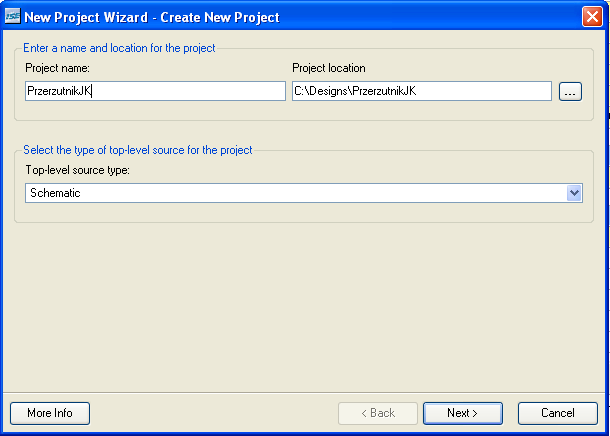
\includegraphics[width=0.49\linewidth]{1.PNG}
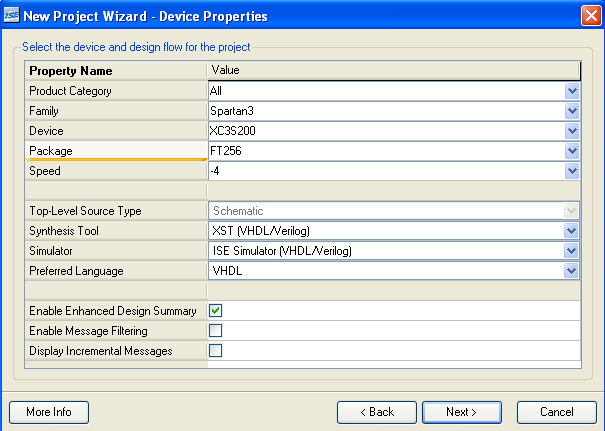
\includegraphics[width=0.49\linewidth]{2.PNG}
} \\
Nacisnąć przycisk Next. Następnie nacisnąć Add Source i wybrać pobrane wcześniej pliki. Następnie nacisnąć kolejne przyciski Next i Finish.
\item Następnie należy utworzyć plik symulacyjny Testbench. Dzięki temu będzie można przetestować zaprojektowany układ przed zaprogramowaniem urządzenia docelowego. Aby to uczynić należy nacisnąć prawy przycisk mysz w miejscu zaznaczonym jak na rysunku i następnie wybrać opcję New Source. W wyświetlonym oknie wybrać opcje tak jak na poniższym rysunku i nadać nazwę pliku. Następnie nacisnąć dwukrotnie przycisk Next oraz na koniec Finish. Wyskoczy kolejne okienko w którym można zmienić parametry zegara takie jak np. jego okres, należy nacisnąć przycisk Finish. \\
\centerline{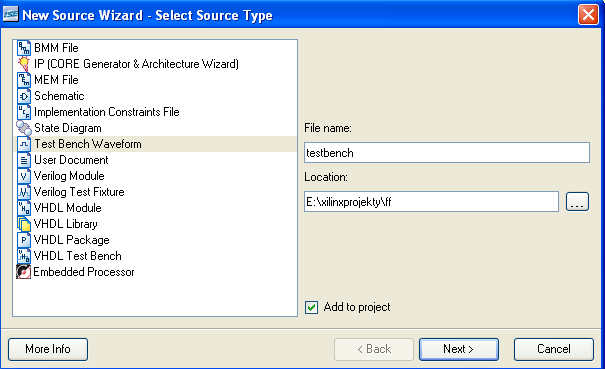
\includegraphics[width=0.5\linewidth]{4.PNG}} \\
\item Można dowolnie ustawić sygnały J oraz K za które odpowiedzialne są przyciski 0 oraz 1. Przycisk 2 służy do resetowania ukladu. Sygnał zmienia się poprzez naciśnięcie na wykresie czasowym w miejscu w którym chcemy aby nastąpiła zmiana.\\
\centerline{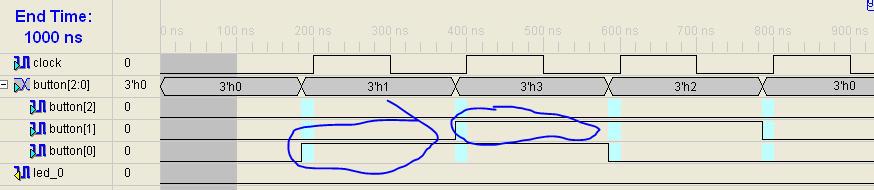
\includegraphics[width=0.8\linewidth]{5.PNG}} \\
Na rysunku zaznaczono miejsca kliknięć.
\item Należy uruchomić symulację poprzez przejście do menu Sources oraz Processes, tak jak zaznaczono na rysunku. A następnie wybranie Behavioral simulation, zaznaczenie pliku Testbench oraz rozpoczęcie symulacji przez dwukrotne kliknięcie we wskazanym miejscu. \\
\centerline{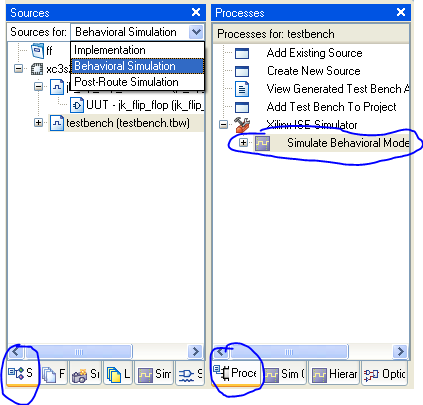
\includegraphics[width=0.5\linewidth]{6.PNG}} \\
\item Jesli wszystko działa poprawnie można przejść do testowania układu bezpośrednio na płytce. Aby to zrobić w okienku Sources należy przejsć do menu Implentation i zaznaczyć nazwę pliku. W okienku Processes należy dwukrotnie nacisnąć Configure Target Device.\\
\centerline{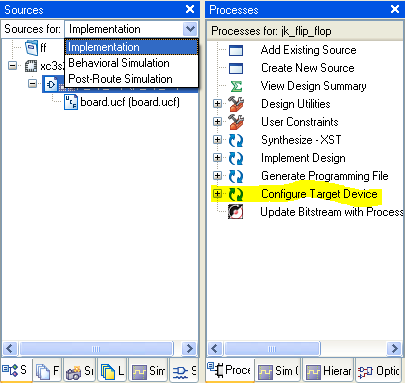
\includegraphics[width=0.5\linewidth]{7.PNG}} \\
Zatwierdzić wywietlony komunikat przyciskiem Ok, a następnie nacisnąć przycisk Finish. W wyświetlonym oknie nalezż wybrać plik z rozszerzeniem .bit i nacisnąć przycisk Open, a w kolejnym nacisnąć Bypass. W okienku które wyskoczy naciskamy przycisk Ok. Ostatnim krokiem jest naciśnięcie prawym przyciskiem w miejscu jak na rysunku oraz wybrać opcję Program. \\
\centerline{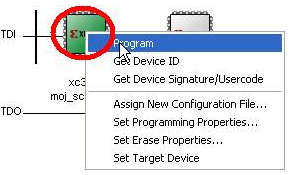
\includegraphics[width=0.5\linewidth]{8.PNG}} \\
\item Można zaobserbować świecenenie diody poprzez naciskanie roznych kombinacji przyciskow, zgodnie z tablicą prawdy przerzutnika JK.
\end{enumerate}
\newpage
\section{Sterownik wyświetlacza siedmiosegmentowego}
\subsection{Teoria}
Kolejnym układem którego działanie zostanie zaprezentowane jest wyświetlacz 7 segmentowy. Taki wyświetlacz, dzięki swojej prostocie, używany jest głównie do wyświetlania liczb. Pojedynczy wyświetlacz składa się z 7 segmentów, które zostają podświetlane zależnie od danych jakie chcemy wyświetlić..(obrazek). W laboratorium występuje  poczwórny wyświetlacz. Taki wyświetlacz posiada jedną 8 bitową linię danych oraz 4 linie aktywujący pojedynczy wyświetlacz. Z tego powodu jeśli na każdym wyświetlaczu chcemy wyświetlić inny znak(np. zrobić stoper) musimy zastosować pewną sztuczkę. Mianowicie dane na każdy z wyświetlaczy należy wysyłać kolejno. Najpierw wysyłamy na pierwszy wyświetlacz, następnie na drugi itp. Aby znak został wyświetlony tylko na jednym wyświetlaczu, na linii aktywującej konkretny wyświetlacz powinna wystąpić wartość 0, a na innych liniach 1. Aby taki układ działał poprawnie, musi działać z pewną częstotliwością. Częstotliwość ta musi być odpowiednio wysoka, aby ludzkie oko nie wychwyciło migotania obrazu. W tym zadaniu została przyjęta 1kHz. Do całości tego zadania został użyty dzielnik częstotliwości z poprzedniego zadania, aby częstotliwość taktowania wyświetlacza nie była zbyt wysoka. 
\newpage
\section{Czasomierz}
\subsection{Teoria}
Lorem ipsum sit dolor amet.
\subsection{Krok po kroku}
Lorem ipsum sit dolor amet.

\newpage
\part{Dodatki}
\end{document}